\chapter{EEG/ERP Portal}


\subsection{About EEG/ERP Portal}

The EEG/ERP Portal is a web-based application which serves to neuroinformatics researchers as a means of managing, sharing and evaluating measured data. The application also comprises advanced featured designed specifically for the needs of EEG/ERP researchers, such as tools for manipulation with EEG signals.


\begin{figure}
	\centering
		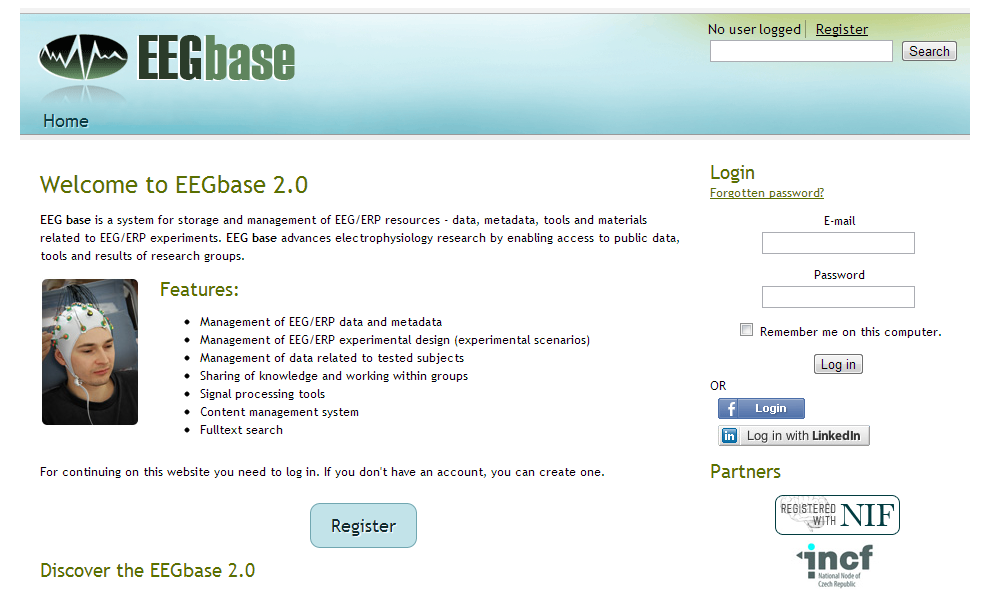
\includegraphics[width=1.00\textwidth]{figures/eegPortal.png}
	\caption{EEG/ERP Portal Welcome Page.}
	\label{fig:eegPortal}
\end{figure}


\subsubsection*{Hibernate}

Hibernate \cite{Hibernate:Home} is an open-source object-relational mapping framework, whose purpose is to facilitate storage and retrieval of Java domain objects. It is used in EEG/ERP Portal

\subsubsection*{Spring Framework}

The Spring Framework facilitates creating Java-based enterprise applications. It applies a principle called dependency injection which helps to make the classes loosely coupled. The idea of this principle is to let the framework do all necessary wiring of objects, so that the objects can focus on their core responsibilities. 

\subsubsection*{Wicket}
... The EEG/ERP Portal's presentation layer is being developed in Wicket by the time of writing this thesis 
